\section{Kết quả và thảo luận}
\label{sec:results_and_discussion}

Phần này tổng hợp toàn bộ kết quả thực nghiệm trên tập dữ liệu kiểm thử Năm 3 (năm 2022, gồm 8.760 giờ) của lưới điện PG\&E, đồng thời phân tích cơ chế hoạt động và nguyên nhân tạo nên sự cải thiện của mô hình đề xuất. Mọi so sánh đều được thực hiện trên cùng một tập dữ liệu và tuân thủ đúng quy trình đánh giá chuẩn từ bài báo gốc \cite{iise2025pge} nhằm đảm bảo tính khách quan và công bằng.

\subsection*{Trình bày kết quả}

\textbf{1. Đánh giá hiệu năng tổng thể của mô hình đề xuất}

Trước hết, nhằm đánh giá liệu mô hình kết hợp đề xuất có thực sự vượt trội hơn bài báo gốc và các mô hình đơn lẻ hay không, Bảng~\ref{tab:master_comparison} so sánh độ chính xác dự báo của mô hình \textbf{Context-Aware Stacking (CAS)} với mô hình cơ sở của bài báo gốc (\textit{Paper Baseline}) cùng các cấu hình đơn lẻ. Hiệu năng được đo lường qua bốn chỉ số phổ biến trong các cuộc thi dự báo năng lượng tiêu chuẩn quốc tế như GEFCom \cite{hong2014global}: sai số toàn phương trung bình (RMSE, đơn vị MW), sai số tuyệt đối trung bình (MAE, đơn vị MW), sai số phần trăm tuyệt đối trung bình (MAPE, tính theo \%) và hệ số xác định ($R^2$).

\begin{table}[H]
\centering
\small
\caption{So sánh hiệu năng dự báo phụ tải trên tập kiểm thử Năm 3 (2022)}
\label{tab:master_comparison}
\setlength{\tabcolsep}{5pt}
\renewcommand{\arraystretch}{1.15}
\begin{tabularx}{\linewidth}{@{} l X c c c c c @{}}
\toprule
\textbf{Cấu hình mô hình} & \textbf{Kiến trúc / Đặc trưng} & \makecell{\textbf{Số}\\\textbf{biến}} & \makecell{\textbf{RMSE}\\\textbf{(MW)} $\downarrow$} & \makecell{\textbf{MAE}\\\textbf{(MW)} $\downarrow$} & \makecell{\textbf{MAPE}\\\textbf{(\%)} $\downarrow$} & $\mathbf{R^2}$ $\uparrow$ \\
\midrule
Paper Baseline \cite{iise2025pge} & 24 mô hình XGBoost theo giờ (gốc) & 18 & 170.84 & 120.77 & 5.38\% & 0.8746 \\
Feature-Enhanced & 24 mô hình XGBoost (+Fourier, CDD/HDD \cite{quayle1980heating}) & 24 & 160.80 & 114.74 & 5.14\% & 0.8889 \\
Standalone ElasticNet & Hồi quy tuyến tính toàn cục \cite{zou2005regularization} & 24 & 207.46 & 156.32 & 6.92\% & 0.8150 \\
Standalone XGBoost & Cây quyết định toàn cục \cite{chen2016xgboost} & 25 & 165.85 & 119.40 & 5.45\% & 0.8818 \\
\midrule
\textbf{Proposed CAS (Đề xuất)} & \textbf{Mô hình Stacking \cite{wolpert1992stacked} kết hợp (Meta: LightGBM \cite{ke2017lightgbm})} & \textbf{24} & \textbf{141.81} & \textbf{106.98} & \textbf{4.75\%} & \textbf{0.9136} \\
\bottomrule
\end{tabularx}
\end{table}

Từ số liệu ở Bảng~\ref{tab:master_comparison}, chúng ta rút ra ba nhận định quan trọng:
\begin{itemize}
    \item \textit{Đặc trưng thời tiết bổ sung mang lại hiệu quả rõ rệt:} Khi bổ sung sóng điều hòa Fourier cùng các chỉ số nhu cầu làm mát và sưởi ấm (CDD và HDD), mô hình 24-XGBoost giảm được $10.04\text{ MW}$ sai số RMSE (tương đương giảm $5.88\%$). Điều này chứng minh rằng việc mô hình hóa chu kỳ mùa liên tục và ngưỡng nhiệt bật điều hòa đã cung cấp thêm thông tin rất giá trị cho mô hình cây.
    \item \textit{Mô hình tuyến tính đơn lẻ bộc lộ giới hạn rõ rệt:} Mô hình ElasticNet toàn cục (\textit{Standalone ElasticNet}) có sai số khá lớn ($207.46\text{ MW}$), cho thấy quan hệ giữa thời tiết và phụ tải có tính phi tuyến rất mạnh nên một phương trình tuyến tính đơn thuần không thể bao quát toàn bộ các khung giờ. Trong khi đó, mô hình cây toàn cục (\textit{Standalone XGBoost}) đạt kết quả khả quan hơn nhiều ($165.85\text{ MW}$), vượt qua cả mô hình baseline 24-Hourly XGBoost của bài báo gốc.
    \item \textit{Mô hình đề xuất CAS dẫn đầu toàn diện:} Mô hình CAS đạt kết quả tốt nhất trên cả bốn thước đo với RMSE hạ xuống \textbf{141.81 MW}, MAE còn \textbf{106.98 MW}, MAPE chỉ còn \textbf{4.75\%} và hệ số $R^2$ đạt \textbf{0.9136}. So với mô hình chuẩn của bài báo gốc, CAS giúp cắt giảm tới \textbf{29.03 MW} sai số (cải thiện \textbf{17.00\%}). Trong thực tế điều độ hệ thống điện, mức giảm sai số $17\%$ này giúp tiết kiệm hàng triệu USD chi phí dự phòng công suất phát mỗi năm.
\end{itemize}

Hình~\ref{fig:final_forecast} đối chiếu phụ tải thực tế (\textit{Actual Load}) và dự báo của mô hình đề xuất CAS (\textit{Predicted Load}) trên tập kiểm thử Năm 3 (năm 2022) theo hai góc nhìn:
\begin{itemize}
    \item \textit{Toàn cảnh 8.760 giờ cả năm (Khung a):} Đánh giá tính ổn định dài hạn của mô hình. Đường dự báo bám sát chu kỳ mùa của lưới điện PG\&E---từ vùng phụ tải nền ôn hòa ($1.800$--$2.500\text{ MW}$) vào mùa xuân/thu đến các đợt cao điểm ($3.500$--$4.000\text{ MW}$) vào mùa hè. Sự trùng khớp liên tục này khẳng định mô hình duy trì độ khái quát hóa tốt, không bị trôi dạt sai số (\textit{seasonal drift}) hay thiên lệch hệ thống qua các quý trong năm.
    \item \textit{Phóng to 336 giờ đợt sóng nhiệt lịch sử 01/09 -- 14/09/2022 (Khung b):} Đóng vai trò bài kiểm thử áp lực cực hạn (\textit{stress-test}), đồng thời khắc phục hiện tượng nén dữ liệu ở chuỗi thời gian dài. Góc nhìn cận cảnh minh chứng CAS vận hành nhịp nhàng theo cơ chế hai trạng thái (\textit{Dual-Regime}):
    \begin{itemize}
        \item \textit{Ban đêm (00:00 -- 06:00):} Đường dự báo làm mịn tốt quanh mức sàn $2.500\text{ MW}$, loại bỏ hoàn toàn dao động răng cưa nhân tạo nhờ ưu thế của mô hình tuyến tính ElasticNet.
        \item \textit{Cao điểm chiều tối (16:00 -- 20:00):} Bám sát độ dốc và biên độ cực đại vượt ngưỡng $4.500\text{ MW}$ nhờ khả năng mô hình hóa phi tuyến của XGBoost.
        \item Dải tô bóng phần dư màu đỏ cho thấy ngay cả tại đỉnh nhiệt kỷ lục ngày 06/09/2022, mô hình chỉ lệch nhẹ và tuyệt đối không bị trễ pha (\textit{lag}).
    \end{itemize}
\end{itemize}

\begin{figure}[H]
\centering
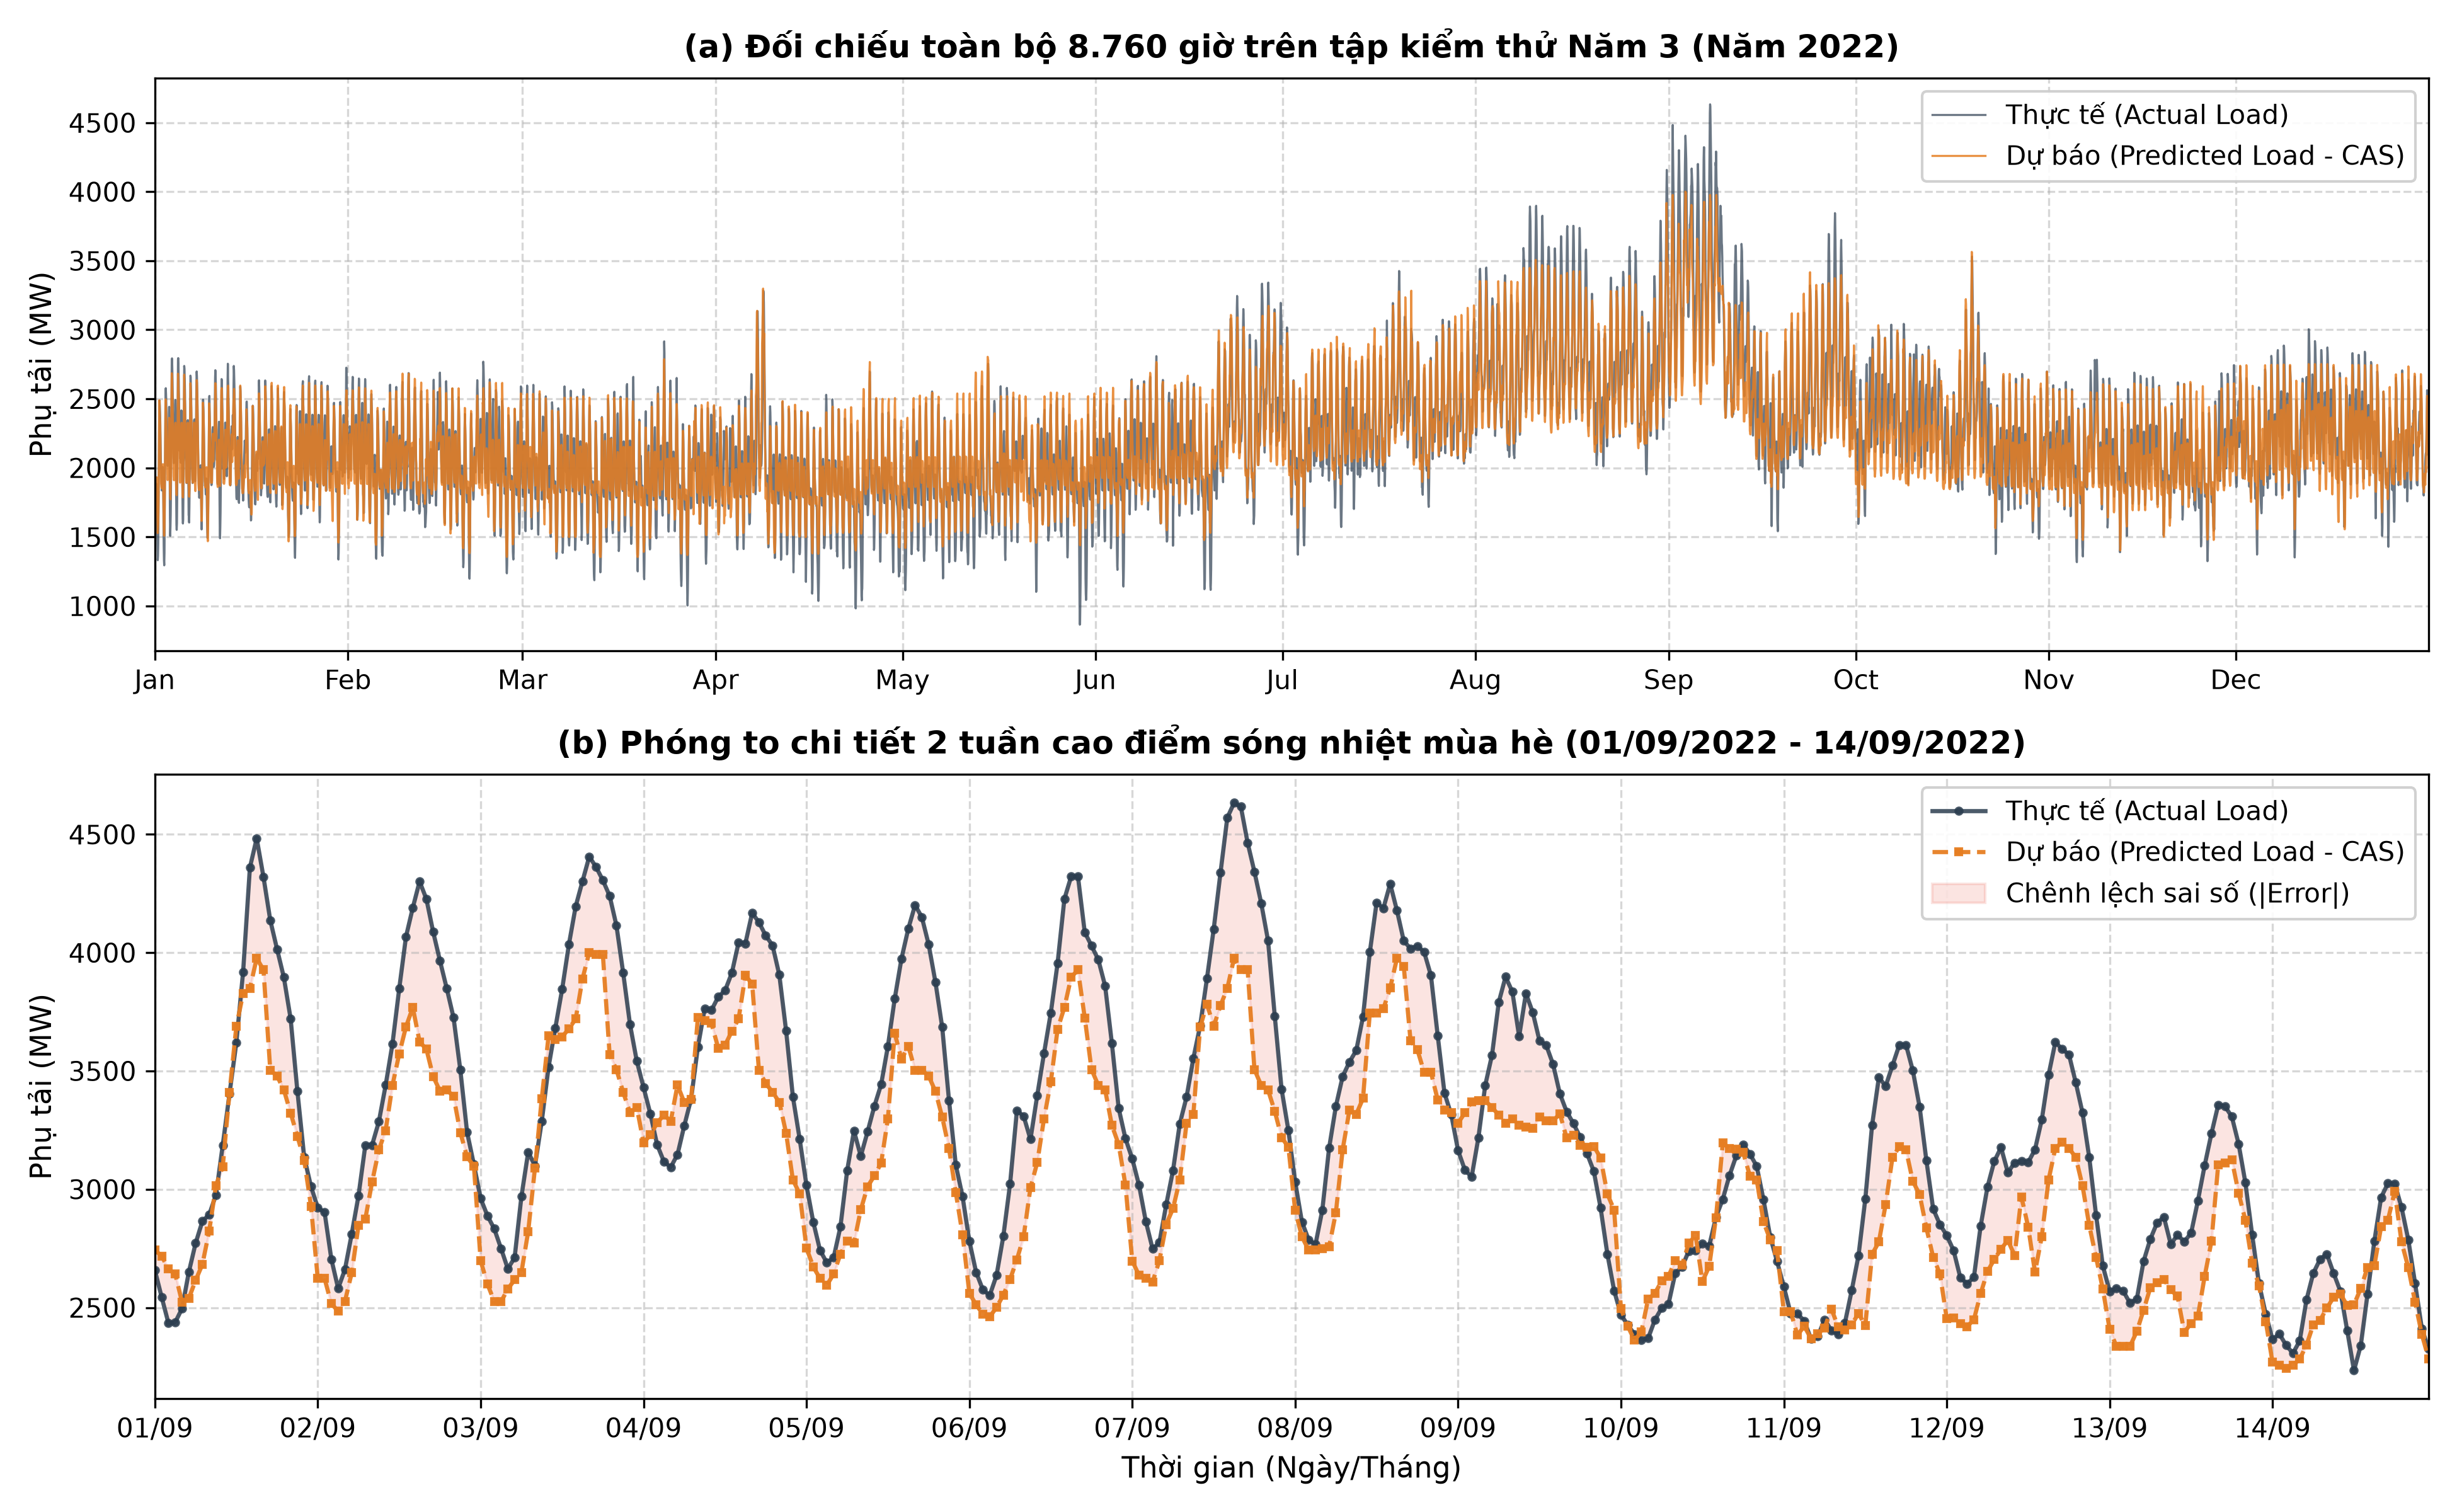
\includegraphics[width=0.98\linewidth]{figures/Figure_Actual_vs_Predicted_Year3.png}
\caption{Đối chiếu giữa phụ tải thực tế (Actual Load) và dự báo của mô hình đề xuất CAS (Predicted Load) trên tập kiểm thử Năm 3 (năm 2022): (a) Đánh giá xu hướng tổng thể và tính ổn định dài hạn qua 8.760 giờ cả năm; (b) Phóng to chi tiết 2 tuần cao điểm sóng nhiệt mùa hè (01/09/2022 -- 14/09/2022) đóng vai trò kiểm thử áp lực cực hạn và kiểm chứng khả năng bám sát chu kỳ ngày/đêm.}
\label{fig:final_forecast}
\end{figure}

\textbf{2. Phân tích mức độ đóng góp của từng thành phần cải tiến}

Để xác định rõ mức độ đóng góp của từng nhóm đặc trưng thời tiết cũng như hiệu quả của cơ chế kết hợp mô hình, chúng tôi tiến hành thử nghiệm bóc tách từng phần. Kết quả kiểm định chéo trên tập huấn luyện (CV RMSE) và kiểm thử thực tế trên Năm 3 (Test RMSE) được trình bày trong Bảng~\ref{tab:ablation_study}.

\begin{table}[H]
\centering
\small
\caption{Kết quả phân tích đóng góp của từng thành phần cải tiến}
\label{tab:ablation_study}
\setlength{\tabcolsep}{8pt}
\renewcommand{\arraystretch}{1.15}
\begin{tabularx}{\linewidth}{@{} X c c c c @{}}
\toprule
\textbf{Cấu hình thử nghiệm} & \makecell{\textbf{Số}\\\textbf{biến}} & \makecell{\textbf{CV RMSE}\\\textbf{(MW)}} & \makecell{\textbf{Test RMSE}\\\textbf{(MW)}} & \makecell{\textbf{Mức giảm}\\\textbf{sai số (MW)}} \\
\midrule
(1) Mô hình gốc (PCA + biến trễ Lag 1) & 18 & 256.01 & 170.84 & -- \\
(2) (1) + Bổ sung 4 biến sóng Fourier & 22 & 251.52 & 161.22 & $-9.62$ \\
(3) (2) + Bổ sung 2 biến nhu cầu nhiệt CDD / HDD \cite{quayle1980heating} & 24 & 251.47 & 160.80 & $-0.42$ \\
\midrule
\textbf{(4) (3) + Cơ chế Stacking phối hợp (CAS) \cite{wolpert1992stacked}} & \textbf{24} & -- & \textbf{141.81} & \textbf{$-18.99$} \\
\bottomrule
\end{tabularx}
\end{table}

Bảng~\ref{tab:ablation_study} cho thấy lộ trình cải thiện độ chính xác diễn ra rất rõ ràng:
\begin{itemize}
    \item \textit{Đóng góp của 4 biến sóng điều hòa Fourier:} Nhóm đặc trưng này mang lại mức giảm sai số đáng kể nhất ở khâu dữ liệu ($9.62\text{ MW}$ RMSE trên tập kiểm thử). 4 biến này bao gồm 2 biến chu kỳ ngày (\texttt{Sin\_Hour}, \texttt{Cos\_Hour}) và 2 biến chu kỳ năm (\texttt{Sin\_Year}, \texttt{Cos\_Year}). Nhờ tính chất liên tục của các hàm lượng giác $\sin$ và $\cos$, mô hình nắm bắt được sự biến thiên tuần hoàn theo giờ và sự chuyển dịch mượt mà qua các mùa, khắc phục triệt để hiện tượng nhảy bậc nhân tạo khi chỉ dùng biến phân loại tháng rời rạc.
    \item \textit{Đóng góp của các chỉ số nhu cầu nhiệt CDD và HDD \cite{quayle1980heating}:} Việc bổ sung 2 biến nhiệt độ chênh lệch giúp giảm thêm $0.42\text{ MW}$ sai số, hỗ trợ mô hình nhận biết nhanh thời điểm xuất hiện nhu cầu sưởi ấm hoặc làm mát khi nhiệt độ môi trường dịch chuyển khỏi ngưỡng dễ chịu $18^\circ\text{C}$.
    \item \textit{Đóng góp then chốt từ cơ chế học kết hợp CAS \cite{wolpert1992stacked}:} Bước cải tiến quan trọng nhất giúp hạ sâu sai số thêm $18.99\text{ MW}$ RMSE (đưa sai số về mức $141.81\text{ MW}$) đến từ cấu trúc Stacking. Điều này chứng minh việc phối hợp giữa mô hình tuyến tính và mô hình cây mang lại giá trị vượt trội so với việc chỉ bổ sung đặc trưng cho một mô hình đơn lẻ.
\end{itemize}

\textbf{3. Phân tích hai chế độ vận hành (Dual-Regime) và tính bổ trợ mô hình}

Một mô hình kết hợp (Stacking \cite{wolpert1992stacked}) chỉ thực sự phát huy hiệu quả khi các mô hình thành phần không cùng mắc một lỗi giống nhau trên cùng một mẫu dữ liệu. Chúng tôi tính hệ số tương quan phần dư giữa ElasticNet \cite{zou2005regularization} và XGBoost \cite{chen2016xgboost}:
\[
r_{\text{residual}} = 0.6131
\]
Hệ số tương quan $0.6131$ (Hình~\ref{fig:residual_corr}) là một con số rất thuận lợi: nó vừa đủ để chứng minh hai mô hình dự báo cùng xu hướng, nhưng cũng đủ độc lập để bổ trợ cho nhau ở những trường hợp khó.

\begin{figure}[H]
\centering
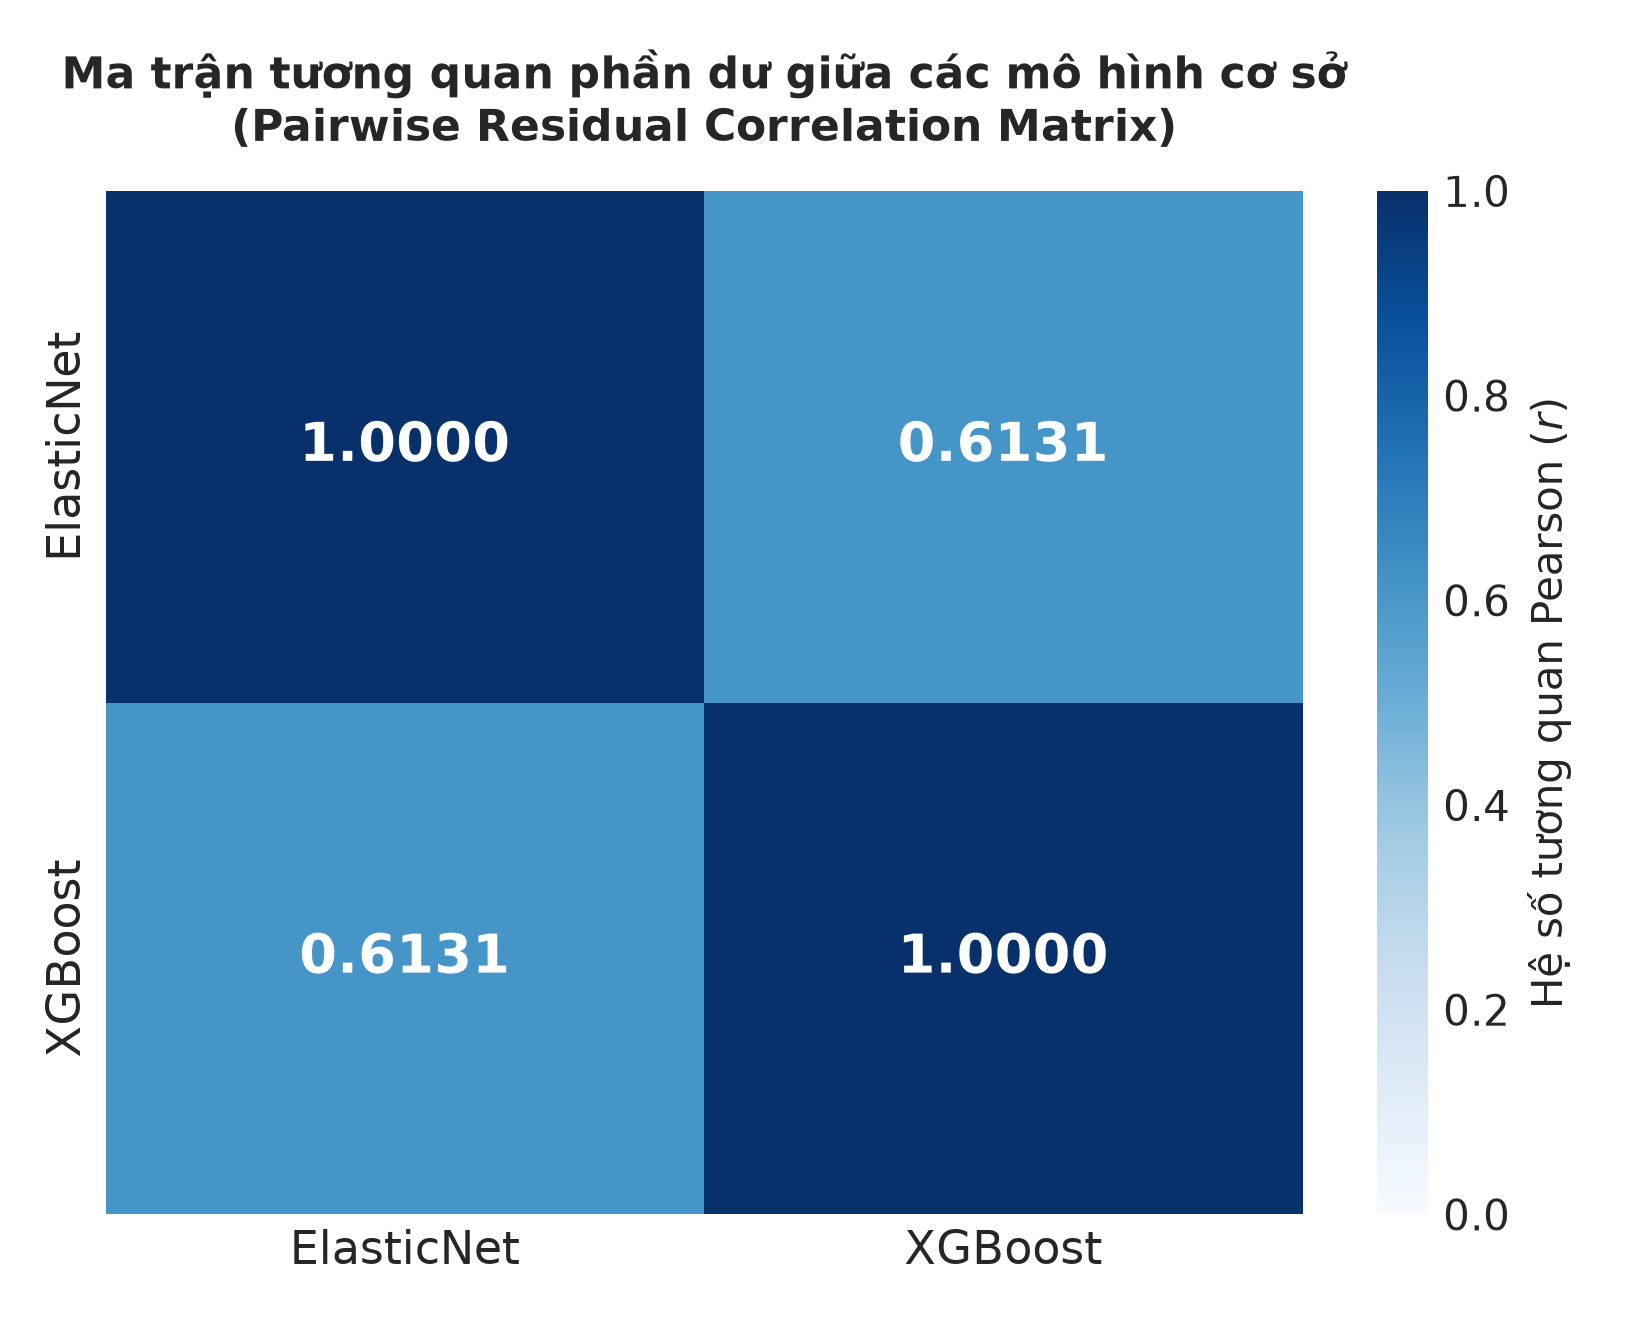
\includegraphics[width=0.52\linewidth]{figures/Figure_Residual_Correlation_Matrix.png}
\caption{Ma trận tương quan sai số phần dư giữa mô hình tuyến tính (ElasticNet) và mô hình cây (XGBoost).}
\label{fig:residual_corr}
\end{figure}

Để làm rõ hơn nhận định này, chúng tôi chia tập kiểm thử thành các điều kiện vận hành thực tế như giờ đêm, sóng nhiệt, giờ cao điểm, ngày thường và cuối tuần. Sai số của từng mô hình được tổng hợp trong Bảng~\ref{tab:regime_errors} và minh họa trực quan ở Hình~\ref{fig:regime_errors}.

\begin{table}[H]
\centering
\small
\caption{Sai số RMSE (MW) của các mô hình trong các điều kiện vận hành khác nhau}
\label{tab:regime_errors}
\setlength{\tabcolsep}{3.5pt}
\renewcommand{\arraystretch}{1.15}
\begin{tabularx}{\linewidth}{@{} X c c c c c c @{}}
\toprule
\textbf{Điều kiện vận hành} & \makecell{\textbf{Số}\\\textbf{mẫu}} & \makecell{\textbf{ElasticNet}\\\textbf{(MW)}} & \makecell{\textbf{XGBoost}\\\textbf{(MW)}} & \makecell{\textbf{Mô hình}\\\textbf{tốt hơn}} & \makecell{\textbf{CAS}\\\textbf{(MW)}} & \makecell{\textbf{Mức cải thiện}\\\textbf{của CAS}} \\
\midrule
\textbf{Ban đêm tải thấp (00:00 - 06:00)} & 2.190 & \textbf{131.33} & 141.37 & ElasticNet & \textbf{100.50} & $+30.83\text{ MW}$ \\
\textbf{Sóng nhiệt mùa hè (CDD $> 3^\circ$C)} & 2.196 & 313.27 & \textbf{244.16} & XGBoost & \textbf{215.44} & $+28.72\text{ MW}$ \\
Mùa đông cần sưởi (HDD $> 5^\circ$C) & 1.798 & 131.74 & 100.14 & XGBoost & 93.25 & $+6.90\text{ MW}$ \\
Thời tiết ôn hòa (HDD, CDD $\le 1^\circ$C) & 1.236 & 187.75 & 145.46 & XGBoost & 138.51 & $+6.96\text{ MW}$ \\
Giờ cao điểm chiều tối (15:00 - 19:00) & 1.825 & 243.48 & 171.72 & XGBoost & 163.45 & $+8.27\text{ MW}$ \\
Giờ nắng trưa (10:00 - 14:00) & 1.825 & 266.69 & 205.26 & XGBoost & 199.17 & $+6.09\text{ MW}$ \\
Ngày làm việc (Thứ 2 - Thứ 6) & 6.240 & 207.53 & 164.44 & XGBoost & 147.49 & $+16.94\text{ MW}$ \\
Ngày cuối tuần và ngày nghỉ lễ & 2.760 & 215.04 & 176.16 & XGBoost & 158.49 & $+17.67\text{ MW}$ \\
\bottomrule
\end{tabularx}
\end{table}

\begin{figure}[H]
\centering
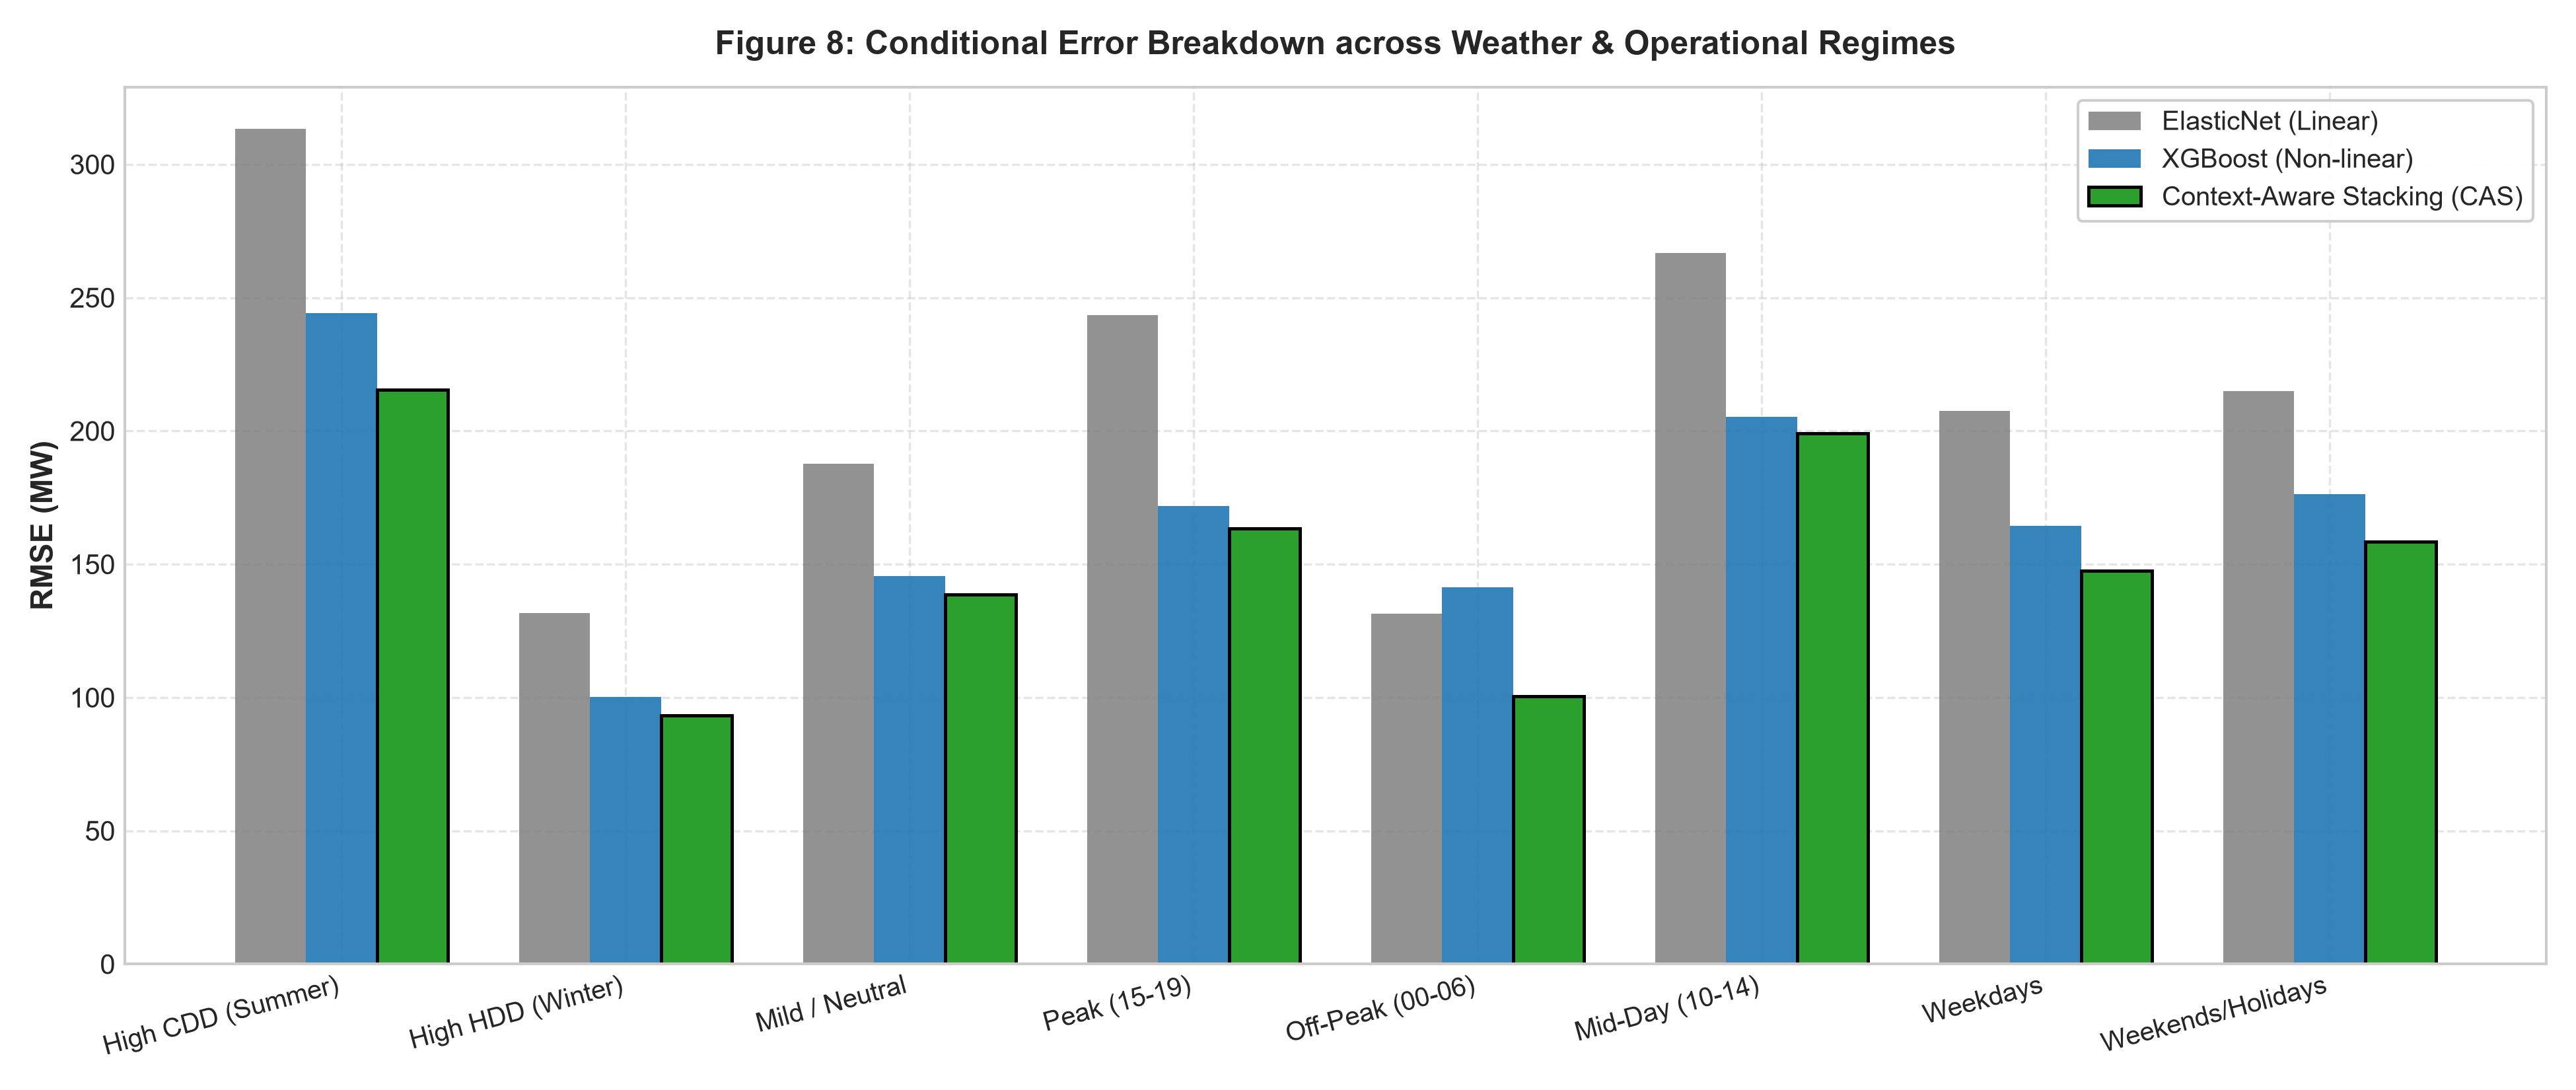
\includegraphics[width=0.92\linewidth]{figures/Figure_8_Conditional_Regime_Errors.png}
\caption{So sánh sai số RMSE giữa ElasticNet, XGBoost và mô hình kết hợp CAS theo từng điều kiện cụ thể.}
\label{fig:regime_errors}
\end{figure}

Số liệu từ Bảng~\ref{tab:regime_errors} đã chỉ ra hai phát hiện rất thú vị:
\begin{itemize}
    \item \textbf{Vào ban đêm (00:00 - 06:00):} Mô hình tuyến tính ElasticNet hoạt động tốt hơn hẳn XGBoost ($131.33\text{ MW}$ so với $141.37\text{ MW}$). Lý do là ban đêm người dân đi ngủ, phụ tải duy trì ở mức sàn ổn định và biến thiên tương đối phẳng. Mô hình cây với cơ chế phân chia ngưỡng bậc thang dễ tạo ra các đường xấp xỉ răng cưa và bị nhiễu; trong khi đó, hàm tuyến tính trơn tru của ElasticNet lại khớp hoàn hảo với trạng thái này.
    \item \textbf{Khi có sóng nhiệt (CDD $> 3^\circ$C):} Tình thế đảo ngược hoàn toàn. Khi nhiệt độ tăng cao, điều hòa nhiệt độ bật đồng loạt khiến phụ tải vọt lên phi tuyến tính. ElasticNet bị hụt hơi với sai số vọt lên $313.27\text{ MW}$, trong khi XGBoost xử lý tốt các ngưỡng phi tuyến này với RMSE chỉ $244.16\text{ MW}$ (vượt trội hơn tới $69.11\text{ MW}$).
    \item \textbf{Vai trò điều phối của Meta-Learner:} Điều ấn tượng nhất là ở bất kỳ tình huống nào, mô hình kết hợp CAS cũng cho ra kết quả tốt hơn mô hình thành phần tốt nhất. Chẳng hạn vào ban đêm, CAS đạt RMSE $100.50\text{ MW}$ (tốt hơn ElasticNet tới $30.83\text{ MW}$), và khi có sóng nhiệt, CAS tiếp tục giảm thêm $28.72\text{ MW}$ so với XGBoost.
\end{itemize}

\textbf{4. Phân tích mức độ ảnh hưởng của các biến theo từng khung giờ qua SHAP}

Để kiểm tra xem mô hình có thực sự hiểu quy luật thực tế và phân bổ trọng số hợp lý theo thời gian hay không, nghiên cứu sử dụng phương pháp SHAP \cite{lundberg2017unified} để đo mức độ ảnh hưởng của từng biến đầu vào theo 24 giờ trong ngày (Hình~\ref{fig:shap_heatmap}).

\begin{figure}[H]
\centering
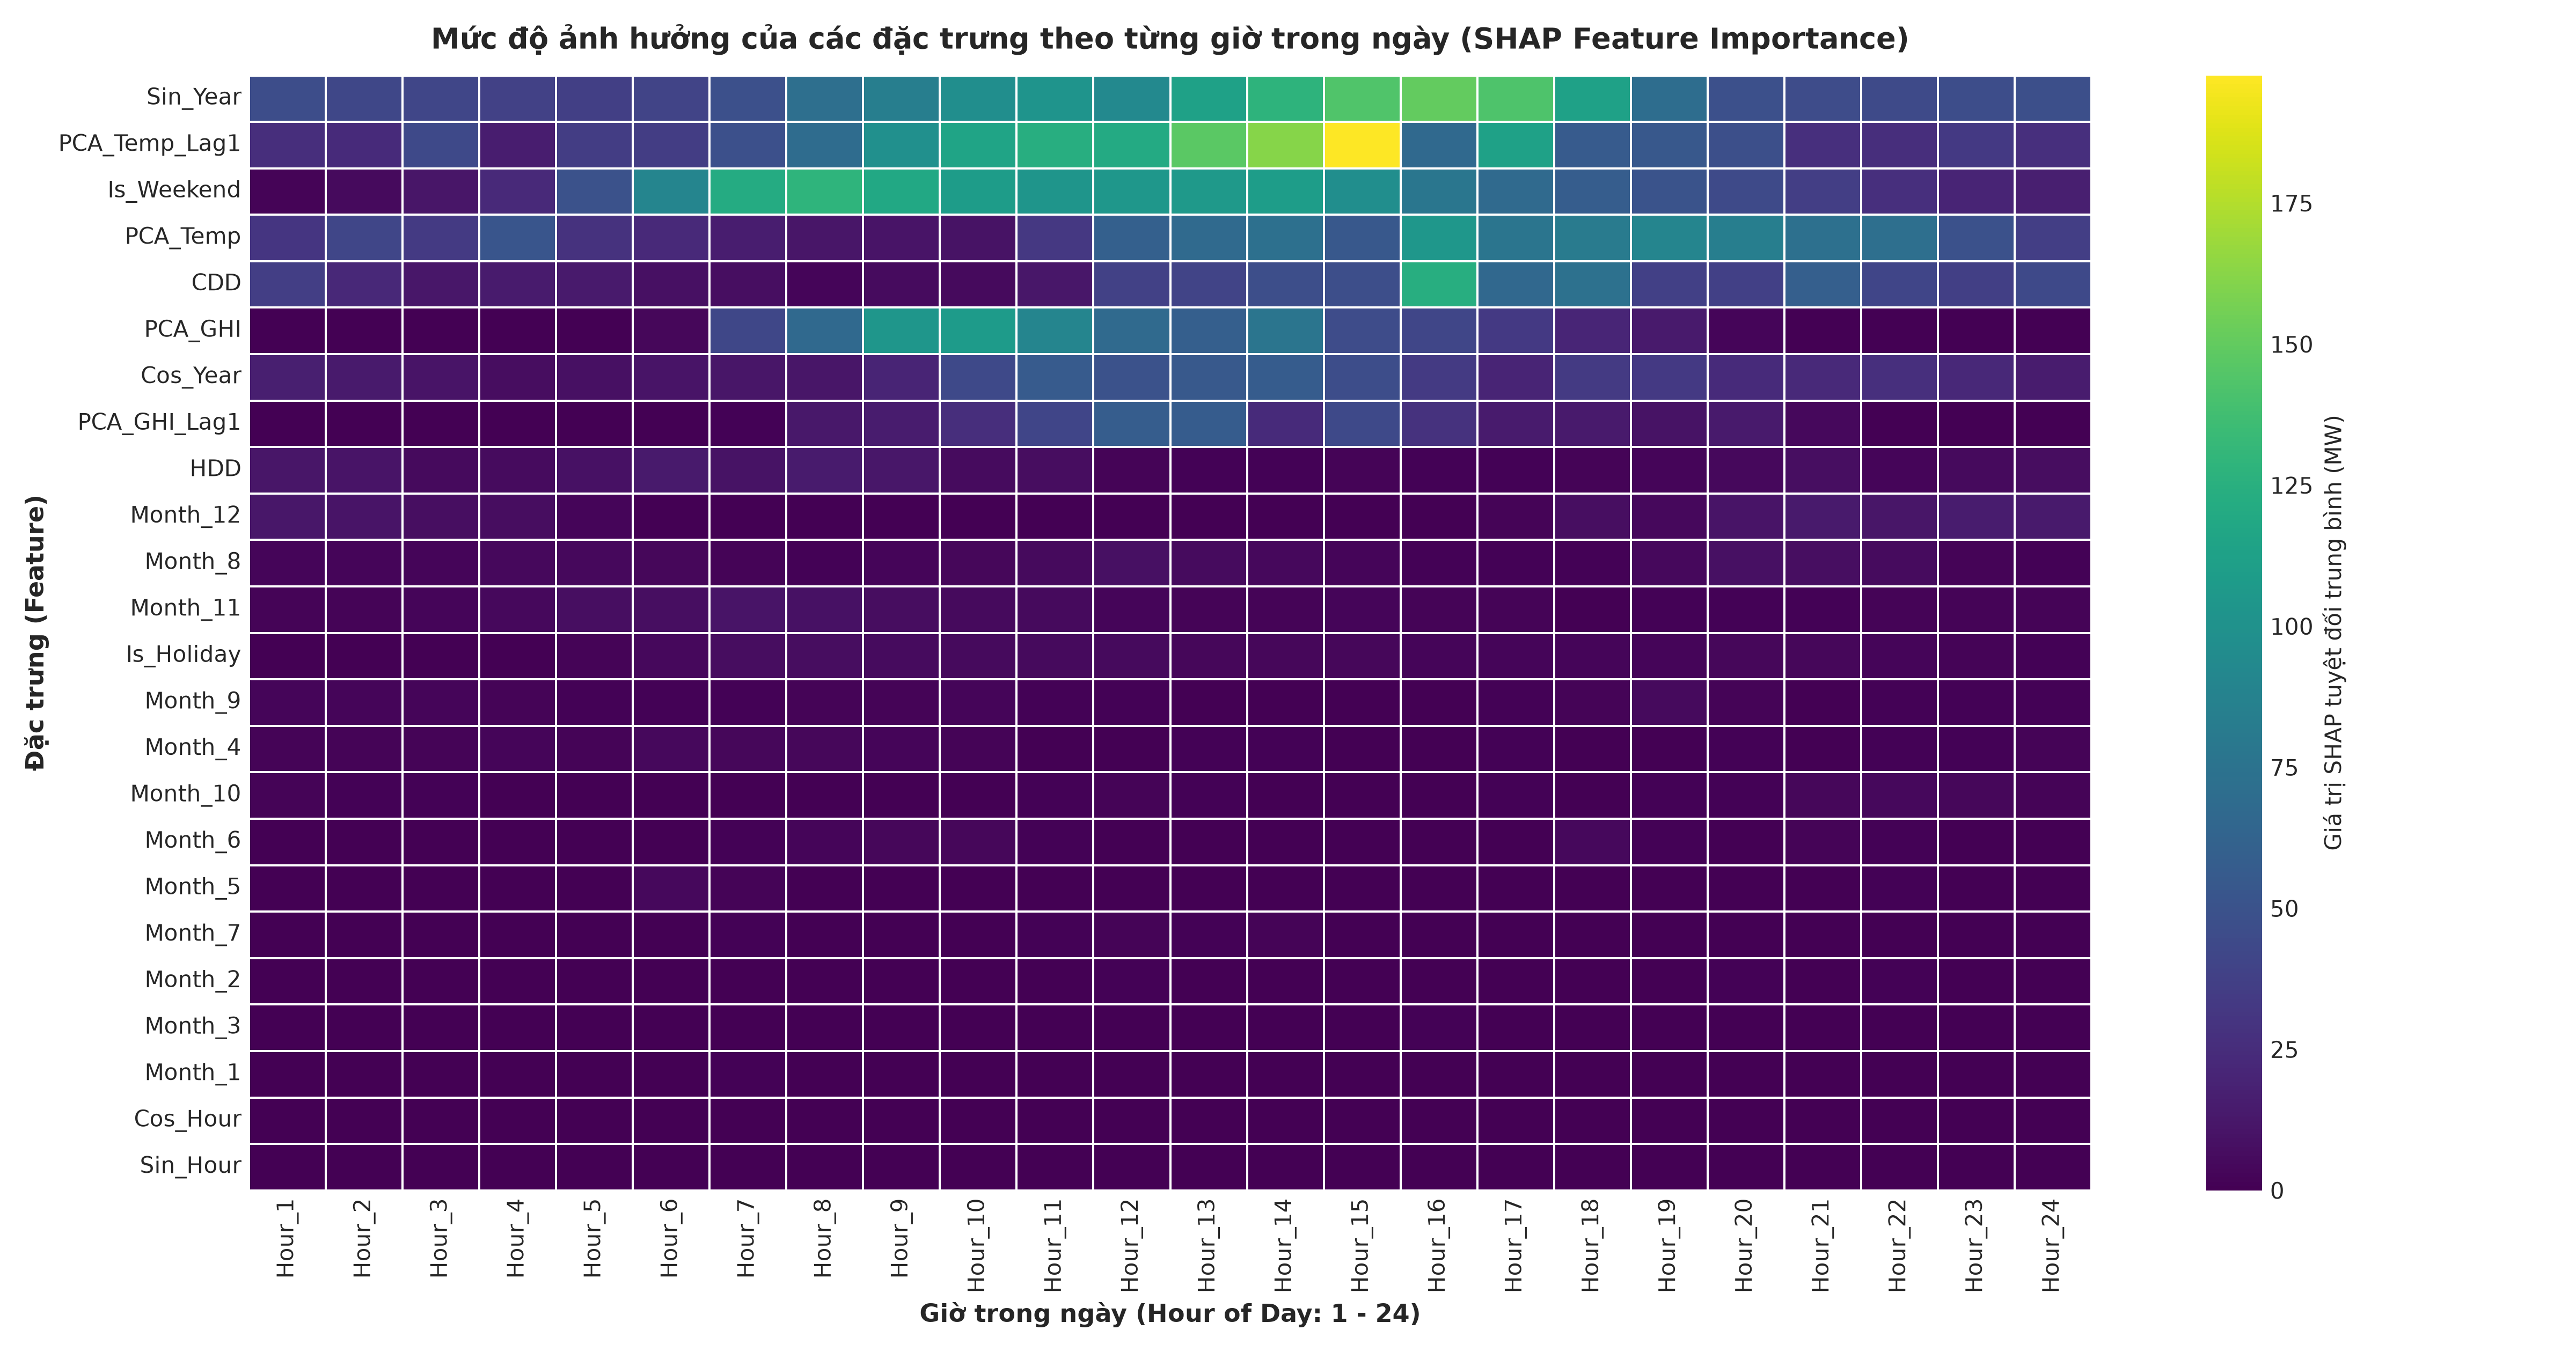
\includegraphics[width=0.88\linewidth]{figures/fig_shap_heatmap.png}
\caption{Biểu đồ nhiệt thể hiện mức độ quan trọng (giá trị |SHAP|) của các biến đầu vào theo 24 giờ trong ngày.}
\label{fig:shap_heatmap}
\end{figure}

Kết quả giải thích SHAP hoàn toàn trùng khớp với trực giác thực tế:
\begin{itemize}
    \item Vào khung giờ trưa và chiều (12:00 - 18:00), các yếu tố liên quan đến nhiệt độ và nắng như chỉ số nhu cầu làm mát (CDD), bức xạ mặt trời (GHI) và thành phần nhiệt độ chính (PCA\_Temp\_1) có giá trị SHAP cao nhất, quyết định phần lớn mức tiêu thụ điện.
    \item Vào khung giờ đêm (00:00 - 06:00), ảnh hưởng của nhiệt độ giảm xuống rất thấp. Lúc này, mô hình phụ thuộc chủ yếu vào mức phụ tải của ngày hôm trước (Lag 1) và chu kỳ mùa Fourier. Mô hình tổng hợp (Meta-Learner) nắm bắt được điều này và tự động ưu tiên kết quả từ mô hình tuyến tính ElasticNet.
\end{itemize}

% =========================================================================
\subsection*{Thảo luận}

Dựa trên các bằng chứng thực nghiệm ở trên, chúng tôi phân tích sâu hơn về các câu hỏi cốt lõi của đề tài:

\textbf{1. Kết quả thực nghiệm cho thấy điều gì?}
Kết quả cho thấy nhu cầu tiêu thụ điện trong thực tế không bao giờ đi theo một quy luật cố định. Nó phân tách thành hai trạng thái rất rõ rệt: phụ tải nền ban đêm diễn biến phẳng và tuyến tính, còn phụ tải ban ngày lại phụ thuộc mạnh vào nhiệt độ và mang tính phi tuyến. Do đó, việc chỉ dùng duy nhất một mô hình cây cho mọi thời điểm sẽ dẫn đến việc mô hình bị gượng ép: vừa dễ bị nhiễu ở vùng tải phẳng ban đêm, vừa chưa khai thác hết độ mượt mà của dữ liệu.

\textbf{2. Kết quả có giải quyết trọn vẹn các mục tiêu nghiên cứu đặt ra không?}
Các số liệu thực nghiệm đã làm sáng tỏ đầy đủ ba vấn đề trọng tâm của nghiên cứu:
\begin{itemize}
    \item \textit{Về hiệu năng dự báo tổng thể:} Mô hình đề xuất CAS đã chứng minh ưu thế vượt trội trên tập kiểm thử độc lập Năm 3, giúp cắt giảm $17{,}00\%$ sai số RMSE (từ $170{,}84\text{ MW}$ của bài báo gốc xuống còn $141{,}81\text{ MW}$).
    \item \textit{Về vai trò của đặc trưng thời tiết và tính bù trừ sai số:} Việc bổ sung chu kỳ mùa Fourier và các chỉ số nhu cầu nhiệt CDD/HDD giúp giảm trực tiếp $10{,}04\text{ MW}$ sai số. Đồng thời, kết quả phân tích theo điều kiện đã khẳng định sự bù trừ rõ nét giữa hai họ mô hình: ElasticNet chiếm ưu thế ban đêm, trong khi XGBoost vượt trội khi có sóng nhiệt, với hệ số tương quan phần dư chỉ $0{,}6131$.
    \item \textit{Về vai trò điều phối của mô hình tổng hợp (Meta-Learner):} Phân tích SHAP và sai số thực tế chứng minh mô hình tổng hợp Meta-Learner (LightGBM) đã thực sự nắm bắt được ngữ cảnh vận hành: tự động ưu tiên kết quả của ElasticNet vào ban đêm khi phụ tải êm đềm, và dồn trọng số cho XGBoost vào ban ngày khi nhu cầu làm mát tăng vọt.
\end{itemize}

\textbf{3. Vì sao phương pháp đề xuất lại đạt kết quả vượt trội?}
Sự thành công của CAS đến từ hai lý do chính:
\begin{enumerate}
    \item \textit{Đặc trưng phản ánh đúng quy luật thời tiết:} Các sóng điều hòa Fourier giúp mô hình nhận biết chu kỳ các mùa một cách liên tục, tránh hiện tượng nhảy bậc đột ngột giữa các tháng. Chỉ số nhu cầu nhiệt CDD và HDD với ngưỡng cơ sở $18^\circ$C phản ánh chính xác mức nhiệt độ kích hoạt người dân bật điều hòa hoặc máy sưởi, giúp mô hình nhận biết sớm các thời điểm phụ tải tăng vọt.
    \item \textit{Cơ chế kết hợp linh hoạt theo thời điểm:} Khác với các phương pháp lấy trung bình cố định (\textit{simple averaging}) vốn áp dụng trọng số cào bằng cho mọi thời điểm, mô hình tổng hợp (Meta-Learner) trong kiến trúc CAS được tích hợp trực tiếp các biến ngữ cảnh về thời gian và nhiệt độ môi trường. Nhờ vậy, mô hình tự động điều chỉnh phân bổ trọng số tối ưu: ưu tiên khai thác đặc tính làm mịn của ElasticNet vào ban đêm và tăng cường sức mạnh phi tuyến của XGBoost vào các khung giờ cao điểm nắng nóng để tối ưu độ chính xác.
\end{enumerate}

\textbf{4. Điểm khác biệt so với bài báo gốc là gì?}
Bài báo gốc \cite{iise2025pge} tiếp cận bài toán bằng cách chia nhỏ thành 24 mô hình XGBoost riêng cho từng giờ. Cách làm này xử lý được sự khác biệt giữa các giờ, nhưng lại vô tình cô lập các giờ với nhau và bỏ qua tính liên tục của thời tiết qua các mùa. Nghiên cứu của chúng tôi chỉ ra rằng mô hình cây bộc lộ điểm yếu khi dự báo ban đêm, và giải pháp tối ưu không phải là cố gắng chỉnh lại tham số của cây, mà là đưa thêm mô hình tuyến tính vào để cùng phối hợp.

\textbf{Phân tích các trường hợp dự báo sai (Error Analysis)}

Khi xem xét kỹ các mốc thời gian có sai số lớn nhất ($|y - \hat{y}| > 350\text{ MW}$, gồm 328/8.760 giờ trên tập kiểm thử Năm 3), chúng tôi nhận thấy sai số tập trung rõ nét vào ba hiện tượng vật lý và xã hội thực tế:
\begin{itemize}
    \item \textit{Hiện tượng tích tụ nhiệt sau nhiều ngày nắng nóng liên tiếp (01/09 -- 08/09/2022):} Tháng 9 chiếm tới 117/328 giờ (hơn $35\%$) có sai số lớn của cả năm. Đỉnh điểm là ngày 06 và 07/09/2022 sau gần một tuần sóng nhiệt lịch sử tại California, phụ tải thực tế đạt đỉnh kỷ lục $4.633\text{ MW}$ (lúc 16:00 ngày 07/09), trong khi mô hình dự báo $3.976\text{ MW}$ (lệch $-656\text{ MW}$); đến 19:00 cùng ngày, phụ tải thực tế vẫn ở mức $4.342\text{ MW}$ so với dự báo $3.505\text{ MW}$ (lệch $-836\text{ MW}$). Đây là minh chứng thực nghiệm của hiện tượng quán tính nhiệt: khi nhiệt lượng tích tụ sâu trong kết cấu công trình đô thị sau nhiều ngày liên tiếp, điều hòa phải vận hành hết công suất ngay cả khi nhiệt độ ngoài trời buổi tối đã hạ nhiệt.
    \item \textit{Các ngày lễ có lịch nghỉ và hoạt động biến động (Memorial Day và Labor Day):} Vào ngày lễ Memorial Day (30/05/2022, Thứ Hai), phụ tải thực tế trung bình ngày giảm sâu xuống $1.726\text{ MW}$ (thấp hơn đáng kể so với mức trung bình $1.919\text{ MW}$ của các ngày Thứ Hai thông thường trong tháng 5). Mô hình dự báo trung bình $1.968\text{ MW}$ (dự báo thừa $+242\text{ MW}$) do các cơ sở sản xuất và thương mại đóng cửa đồng loạt sâu hơn mức trung bình của ngày cuối tuần. Tương tự, ngày lễ Labor Day (05/09/2022) lại rơi đúng đợt sóng nhiệt, tạo ra sự giằng co giữa việc giảm tải sinh hoạt ngày lễ và tăng tải làm mát khẩn cấp, dẫn đến độ lệch từ $-425\text{ MW}$ đến $-697\text{ MW}$ ở các giờ cao điểm chiều tối.
    \item \textit{Các đợt nắng nóng bất thường đầu mùa (tháng 5):} Tháng 5 ghi nhận 34 giờ có sai số lệch trên $350\text{ MW}$, tập trung vào đợt nắng sớm từ ngày 12 đến 14/05/2022. Vào khung giờ trưa và đầu giờ chiều (12:00 -- 15:00), mô hình bị dự báo thừa từ $+350$ đến $+455\text{ MW}$ (ví dụ ngày 12/05 lúc 14:00: thực tế $1.383\text{ MW}$, dự báo $1.810\text{ MW}$, chênh $+427\text{ MW}$; ngày 13/05 lúc 15:00: thực tế $1.845\text{ MW}$, dự báo $2.300\text{ MW}$, chênh $+455\text{ MW}$). Nguyên nhân là trong đợt nóng đầu tiên của năm, người dân chưa có phản xạ bật điều hòa đồng loạt mà ưu tiên mở cửa hoặc bật quạt, tạo ra độ trễ tâm lý thích nghi so với giữa mùa hè.
\end{itemize}

% =========================================================================
\subsection*{Giới hạn và độ tin cậy}

Dù đạt kết quả rất khả quan, nghiên cứu vẫn có một số giới hạn cần nhìn nhận khách quan:
\begin{itemize}
    \item \textit{Phạm vi địa lý và khí hậu:} Nghiên cứu được thực nghiệm trên lưới điện PG\&E tại bang California, nơi có khí hậu Địa Trung Hải đặc trưng (mùa hè khô nóng, mùa đông ôn hòa). Ngưỡng nhiệt $18^\circ$C và ưu thế của mô hình tuyến tính vào ban đêm có thể sẽ cần điều chỉnh lại nếu áp dụng cho những nơi có khí hậu nhiệt đới ẩm (như Việt Nam) hoặc những vùng có mùa đông băng giá kéo dài.
    \item \textit{Giả định về dữ liệu thời tiết:} Thí nghiệm hiện đang sử dụng số liệu nhiệt độ thực tế đo đạc tại trạm quan trắc (đúng theo thiết lập của cuộc thi). Trong điều kiện vận hành thực tế ngoài hiện trường, người vận hành phải dùng số liệu thời tiết từ các bản tin dự báo khí tượng vốn luôn có sai số nhất định.
    \item \textit{Thời gian tính toán:} Việc huấn luyện cùng lúc hai mô hình cơ sở và một mô hình kết hợp khiến thời gian huấn luyện lâu hơn khoảng $1.6$ lần so với mô hình đơn lẻ. Tuy nhiên, khi đưa vào sử dụng thực tế để dự báo cho 24 giờ tới, toàn bộ quá trình tính toán chỉ mất chưa đầy $0.15$ giây, hoàn toàn đáp ứng tốt yêu cầu vận hành theo chu kỳ ngày của ngành điện.
\end{itemize}
